
\documentclass[a4paper]{article}\usepackage[]{graphicx}\usepackage[]{color}
%% maxwidth is the original width if it is less than linewidth
%% otherwise use linewidth (to make sure the graphics do not exceed the margin)
\makeatletter
\def\maxwidth{ %
  \ifdim\Gin@nat@width>\linewidth
    \linewidth
  \else
    \Gin@nat@width
  \fi
}
\makeatother

\definecolor{fgcolor}{rgb}{0.345, 0.345, 0.345}
\newcommand{\hlnum}[1]{\textcolor[rgb]{0.686,0.059,0.569}{#1}}%
\newcommand{\hlstr}[1]{\textcolor[rgb]{0.192,0.494,0.8}{#1}}%
\newcommand{\hlcom}[1]{\textcolor[rgb]{0.678,0.584,0.686}{\textit{#1}}}%
\newcommand{\hlopt}[1]{\textcolor[rgb]{0,0,0}{#1}}%
\newcommand{\hlstd}[1]{\textcolor[rgb]{0.345,0.345,0.345}{#1}}%
\newcommand{\hlkwa}[1]{\textcolor[rgb]{0.161,0.373,0.58}{\textbf{#1}}}%
\newcommand{\hlkwb}[1]{\textcolor[rgb]{0.69,0.353,0.396}{#1}}%
\newcommand{\hlkwc}[1]{\textcolor[rgb]{0.333,0.667,0.333}{#1}}%
\newcommand{\hlkwd}[1]{\textcolor[rgb]{0.737,0.353,0.396}{\textbf{#1}}}%

\usepackage{framed}
\makeatletter
\newenvironment{kframe}{%
 \def\at@end@of@kframe{}%
 \ifinner\ifhmode%
  \def\at@end@of@kframe{\end{minipage}}%
  \begin{minipage}{\columnwidth}%
 \fi\fi%
 \def\FrameCommand##1{\hskip\@totalleftmargin \hskip-\fboxsep
 \colorbox{shadecolor}{##1}\hskip-\fboxsep
     % There is no \\@totalrightmargin, so:
     \hskip-\linewidth \hskip-\@totalleftmargin \hskip\columnwidth}%
 \MakeFramed {\advance\hsize-\width
   \@totalleftmargin\z@ \linewidth\hsize
   \@setminipage}}%
 {\par\unskip\endMakeFramed%
 \at@end@of@kframe}
\makeatother

\definecolor{shadecolor}{rgb}{.97, .97, .97}
\definecolor{messagecolor}{rgb}{0, 0, 0}
\definecolor{warningcolor}{rgb}{1, 0, 1}
\definecolor{errorcolor}{rgb}{1, 0, 0}
\newenvironment{knitrout}{}{} % an empty environment to be redefined in TeX

\usepackage{alltt}

%--- Load packages. 
\usepackage{amssymb,amsmath}
\usepackage{framed}

% avoid ugly indentation of paragraphs
\usepackage{parskip}
\usepackage{graphicx}

% open sans font
\usepackage[default,osfigures,scale=0.95]{opensans}

% subfolder with the figures (within manuscript/)
\graphicspath{ {./figures/} }

% for author affiliations
\usepackage{authblk}

%allows inline citations
%\usepackage[round]{natbib}
%\bibliographystyle{plainnat}

% for degree symbol
\usepackage{gensymb}

% for line numbers
\usepackage{lineno}

% margin size
\usepackage{geometry}
\geometry{verbose,tmargin=3cm,bmargin=3cm,lmargin=3cm,rmargin=3cm}

% for bibtex
\usepackage{authordate1-4}
\bibliographystyle{authordate1}

%allows subscripts in text mode
\usepackage{fixltx2e}
\IfFileExists{upquote.sty}{\usepackage{upquote}}{}
\begin{document}


\title{Effects of belowground space limitation on performance of Eucalyptus seedlings:  Does photosyntheis really control growth?}

\author[1,3]{Courtney E. Campany}
\author[2]{Belinda E. Medlyn}
\author[1]{Remko A. Duursma}

\affil[1]{Hawkesbury Institute for the Environment, University of Western Sydney, Richmond, NSW 2753, Australia}
\affil[2]{Department of Biological Sciences, Macquarie University, North Ryde, NSW 2109, Australia}
\affil[3]{Corresponding author (c.campany@uws.edu.au)}

\renewcommand\Authands{ and }
\maketitle


%--------------------------------------------------------------------------------------------%

\section*{Abstract}

Negative feedbacks to photosynthesis are commonly interpreted as the primary factor responsible for growth limitation in plants under stress.  This study used manipulations of soil volume to test how growth is coupled to physiology, allocation, and sink activity in Eucalyptus tereticornis seedlings. We grew seedlings in a large range of container sizes and planted containers flush to the soil alongside freely rooted seedlings (‘free’). Reduced soil volume was expected to induce rapid negative effects on growth and physiology compared to free seedlings. It was hypothesized that soil volume effect would be largest in the smallest containers, resulting in physical constraints to growth independently of photosynthesis. Photosynthesis would then become sink-limited, resulting in the build-up of leaf nonstructural carbohydrates eventually leading to photosynthetic down regulation. We observed a negative container effect on aboveground growth soon after the experiment started. Although growth was consistently different across soil volumes mass allocation to leaves, stems, roots was conserved after 120 days. Photosynthetic capacity was also significantly reduced in containers, and was related to both leaf nitrogen content and starch accumulation, however starch effects were weaker. We developed a simple seedling growth model that utilized leaf photosynthesis rates to allocate daily carbon (c) uptake towards mass growth of stems, leaves and roots. We then asked whether the observed reductions in photosynthesis explained the observed differences in seedling biomass.  We found that photosynthesis reductions alone was not sufficient and the inclusion of mass allocation patterns and additional C pools were necessary to predict the observed growth response to increasing soil volume. Overall, we found limited evidence for sink-limitation of photosynthesis by constraining seedling growth in containers, and argue that shifts in C allocation are necessary to explain the experimental results. This research highlights the need to further understand adaptive strategies of plant C allocation, and confirms that photosynthesis and growth are not always directly related.

\section*{Key Words}

photosynthesis, sink regulation, growth, carbon allocation, soil volume


\section*{Introduction}

\section*{Methods}

\subsection*{\textit{Experimental Design}}

This experiment was located on the Hawkesbury Forest Experiment site in Richmond, NSW, Australia. Plots were located in open cover with a site history that consists of a paddock that was converted from native pasture grasses. Top soils at this site, used for the study, are an alluvial formation of low-fertility sandy loam soils (380 and 108~mg~kg\textsuperscript{-1} total N and P respectively) with low organic matter (0.7\%) and low water holding capacity. At this site a soil hard layer exists at $\sim$1.0~m with a transition to heavy clay soils. The climate for the region is classified as sub-humid temperate. 

\textit{Eucalyptus tereticornis} seedlings, 20~weeks old and approximately 40~cm tall in tube stock, were chosen from a single local Cumberland plain cohort. Previous experiments have confirmed that species with tap roots (similar to \textit{E. tereticornis}) use the center of the container as the medium for thick roots leaving the periphery of the soil as the most active sites for fine root proliferation \cite{biran1980a,biran1980b}. This is generally hypothesized to be a different response than seedlings with no taproot. By using a species with tap root growth and manipulations of container length rather than width, it is believed that a more realistic test of inhibition of growth through constrained soil volume would be achieved. Six seedlings were harvested before planting to measure initial leaf area and dry mass of leaves, stems and roots.

Six container volumes were used ranging from 5~l to 3~l, with a 22.5~cm diameter, and lengths ranging from 15 to 100~cm. Containers were constructed of PVC pipe and were filled with local top soil (described above). Soil in each container was packed to achieve a target soil bulk density of 1.7~g~m\textsuperscript{-3}. Each seedling was given an Imidacloprid (BAYER CropScience) insecticide tablet planted 5 cm below the roots. Containers were planted flush with the soil surface inside metal sleeves, designed to minimize excess air space between the container and outside soil while allowing container removal. This allowed for soil temperatures in containers to reflect conditions of naturally sown seedlings. Each experimental block (n=7) contained a complete replicate set of container volumes as well as one ‘free’ seedling, with 1 m\textsuperscript{2} spacing. For each ‘free’ seedling, a 1~m\textsuperscript{2} subplot was excavated to 0.5 m and replaced with the same soil used in each container. A border of root exclusion material was buried 0.25 m deep and extended 0.25~m above the ground surface to exclude local vegetation.

Plants were watered bi-weekly or when needed, accounting for natural precipitation, to maintain soil moisture at field capacity (13-15~\%). To achieve field capacity all soil filled containers were weighed and soil moisture was measured (Time Domain Reflectometer at 10~cm depth) before watering. Derived equations based on container weight at planting (when soil moisture was 3~\%) and at field capacity was used to calculate watering requirements for each individual plant. Drain systems were built into each pot to prevent pooling of water in containers before root expansion, from reduced root uptake, or from large rainfall events. These conditions could lead to an anaerobic environment around the root that could hinder the uptake of water through reduced root conductance \cite{poorter2009causes}, an undesired experimental artifact. A collection compartment in the bottom of containers, containing gravel covered by root exclusion mesh, was used collect water for 20, 25, and 35~l containers. Plastic tubing (6 mm diameter) was inset into the gravel layer and extended through the top of the container. A lysimeter pump was then used to suction excess water, through the tubing, as needed. As small containers (5, 10, and 15~l) have a larger irradiation effect a simple bottom plug was used to drain water from the gravel compartment.  

\subsection*{\textit{Growth and morphology metrics}}
Seedlings were planted on January 21\textsuperscript{st} 2013 and stem height, diameter at 15~cm and leaf count were measured weekly thereafter. Once the growth rate of individual plants had significantly declined a full biomass harvest was completed (May 5\textsuperscript{th} 2013). Dry mass of leaves, stems, roots and cumulative leaf area (LI-3100C Area Meter; LI-COR, Lincoln, NE, USA) was measured for each seedling. Mean individual leaf area for each harvested seedling was calculated by dividing cumulative leaf area by total leaf count of only fully expanded leaves. This value was then used to interpolate cumulative leaf area through time with weekly leaf counts. Root mass was collected by passing soil from each container through a 1 mm sieve, washing, separating into fine and coarse roots (\textless2~mm and \textgreater2~mm diameter, respectively) and then drying to a constant mass. Roots from the ‘free’ seedlings were collected by excavating each 1~m\textsuperscript{2} subplot to 0.5~m depth.  25~g fresh weight subsamples of washed fine roots were analyzed, using WhinoRhizo software (Regent Instruments Inc.), for specific root length (SRL, m~m\textsuperscript{-1}).

\subsection*{\textit{Photosynthetic parameters}}
Leaf gas exchange measurements were performed bi-weekly at saturating light (A\textsubscript{sat}) and saturating light and [CO\textsubscript{2}] (A\textsubscript{max}) on new fully expanded leaves. Measurements were initiated only after new leaf growth occurred (March 17\textsuperscript{th}, 2013), approximately 6 weeks following planting, and continued until the biomass harvest. Leaf level gas exchange was measured with a standard leaf chamber equipped with blue-red light emitting diodes using a portable gas exchange system (LI-6400, LI-COR, Lincoln, NE, USA). A\textsubscript{sat} measurements were made at PPFD of 1800~$\mu$mol~m\textsuperscript{-1}~s\textsuperscript{-1} and [CO\textsubscript{2}] of 400~$\mu$l~l\textsuperscript{-1} and A\textsubscript{max} with [CO\textsubscript{2}] of 1600~$\mu$l~l\textsuperscript{-1} and PPFD of 1800~$\mu$mol~photons~m\textsuperscript{-1}~s\textsuperscript{-1}. This choice of light level to achieve light saturation is consistent with other studies on \textit{Eucalyptus} species \cite{kallarackal1997ecophysiological,pinkard1998photosynthetic,crous2013photosynthesis,drake2014capacity}. These measurements were conducted during midday (10:00-14:00~h) with leaf temperature maintained at 25$\degree$C. After leaves acclimated to the chamber environment, net CO\textsubscript{2} assimilation rate and stomatal conductance were logged 5 times for both A\textsubscript{sat} and A\textsubscript{max}. Photosynthetic CO\textsubscript{2} response (AC\textsubscript{i}) curves were also constructed on a random subset of each container size (n=3) after new leaves were first produced and immediately prior to the final harvest (May 23\textsuperscript{rd} 2013). For each AC\textsubscript{i} curve the reference [CO\textsubscript{2}] was set as follows:  400, 50, 100, 150, 230, 330, 400, 650, 900, 1200, 1500, 1600, and 1800~$\mu$l~l\textsuperscript{-1}. From these curves the photosynthetic parameters, J\textsubscript{max} and V\textsubscript{cmax}, were quantified using the leaf photosynthesis model by farquhar1980biochemical and a Ball-Berry type model of stomatatal conductance ()within the 'plantecophys' package in R v. 3.0.1 \cite{plantecophys,RDevelopmentCoreTeam2011}.  Leaf dark respiration rates (R\textsubscript{d}) was measured on each seedling during the same dates as AC\textsubscript{i} curves using detached leaves inside a conifer chamber attached to the Licor 6400 at least 1 hour after sundown.   Measurements were taken at a reference [CO\textsubscript{2}] of 400~$\mu$l~l\textsuperscript{-1} while leaf temperature was maintained at current ambient conditions. Specific leaf area (SLA, m\textsuperscript{2}~g\textsuperscript{-1}) was calculated by measuring leaf area and dry mass for all leaves sampled during gas exchange campaigns.

\subsection*{\textit{Leaf water potential}}
Predawn ($\Psi\textsubscript{pd}$) and midday ($\Psi\textsubscript{l}$) water potentials were measured for each seedling using a PMS 1505D pressure chamber (PMS Instruments, Albany, OR, USA) on fully expanded leaves during the same time period as AC\textsubscript{i} and (R\textsubscript{d}). $\Psi\textsubscript{pd}$ and $\Psi\textsubscript{l}$ leaves were sampled and immediately stored inside foil covered bags and then transported to the laboratory for measurements of water potential. $\Psi$ collections were completed before sunrise and midday 13:00-14:30~h. These measurements were used as a measure of static water stress on the seedlings \cite{sellin1999does}, and to ensure that the bulk soil water availability was high enough for plants as they became larger and roots filled the soil volume. 

\subsection*{\textit{Leaf, root and soil chemistry}}
Leaves used in each gas exchange measurement and subsamples of harvested fine roots were dried to a constant mass and milled for analysis of N and C content. Pre-planting soil samples (n=6) and subsamples of soil from each container following harvest were sieved to remove organic material, air dried and milled for analysis. C and N concentrations of milled samples were determined using a Carlo Erba CE1110 elemental analyzer with thermal conductivity and mass spectromic detection (of N\textsuperscript{2} and CO\textsubscript{2}).  The percentage of N and C in the sample was calculated by comparison with known standards. Leaf total non-structural carbohydrates concentration (TNC) was analyzed using a total starch assay kit (Megazyme International 303 Ireland Ltd., Wicklow, Ireland) on gas exchange leaves (above) and represents the sum of starch (mg~g\textsuperscript{-1}) and soluble sugar (mg~g\textsuperscript{-1}) concentrations. Starch was quantified using a thermostable $\alpha$-amylase and amyloglucosidase assay \cite{MCCLEARY} and soluble sugars were determined following the anthrone method /cite{ebell1969variation}. Full methods of the TNC assay are described in \cite{mitchell2013drought}.

\subsection*{\textit{Seedling growth model}}
We developed a simple seedling growth model that utilized leaf photosynthesis to allocate daily carbon assimlate towards mass production of stems, leaves and roots. The model starts with mean initial seedling mass (leaf\textsubscript{0}, stem\textsubscript{0} and root\textsubscript{0}) and a starting leaf area (LA\textsubscript{0}) measured prior to planting. Biomass production for each day of the experiment was estimated by multiplying the whole tree seedling carbon uptake gain per day (C\textsubscript{day}) by a biomass conversion efficiency parameter ($\xi\textsubscript{c}$, \cite{zhu2008maximum}), allocating new carbon to the previous day’s biomass and then accounting for carbon loss via tissue respiration. C\textsubscript{day} was calculated for each seedling by fitting a coupled photosynthesis - stomatal conductance model \cite{farquhar1980biochemical,farquhar1982stomatal,medlyn2002temperature} in the 'plantecophys' package in R \cite{plantecophys} to the mean photosynthetic parameters (R\textsubscript{d}, J\textsubscript{max}, V\textsubscript{cmax}, and g\textsubscript{1}) generated for each soil volume and meteorological data from an onsite weather station.  The g\textsubscript{1} parameter was generated by fitting observed stomatal conductance values into the optimal stomatal conductance model from \cite{medlyn2012reconciling}.  Combined with the meteorological parameters PPFD, air temperature, and relative humidity, at 15~m intervals, photosynthesis rates ($\mu$mol~CO\textsubscript{2}~m\textsuperscript{-2}~s\textsuperscript{-1}) were then predicted for each soil volume treatment. Rates were assumed to be representative of the entire 15~min meteorological interval. C\textsubscript{day} was then calculated by converting predicted rates to mass carbon gain over 15~min (g~m\textsuperscript{-2}) and then summed for 24~h. Additionally, it was necessary to calculate a self-shading parameter (M) when scaling flat leaf photosynthesis to seedling cumulative leaf area.  This was accomplished by utilizing 61 previously digitized Eucalyptus seedlings (\textit{E. tereticornis, E. haemastoma, E. pilularis, E. saligna}) from published studies (cites) run in 'YplantQMC' package in R \cite{yplantqmc} to build a 3d plant structure based on digitized metrics of plant allometry and crown structure. Inputting the same physiological parameters listed above, 'YplantQMC' outputs total photosynthesis, using total leaf area, for seedlings assuming self-shading as well as for a full sun large horizontal leaf.  The ratio of self-shading to flat leaf total photosynthesis was then used to calculate M, which was then applied to modelled rates of photosynthesis when scaling to seedling cumulative leaf area. All parameters used in model simulations are reported in Table 2

We then utilized this model to to investigate whether the effects of soil volume on photosynthesis were enough to accurately predict overall seedling production after 120 days or whether changes in carbon allocation or mass partitioning where also necessary to predict biomass. First, the model was simulated using only changes in photosynthesis rates across treatments combined with mean values of mass partitioning and either published or local data of stem and root respiration rates. Next, different mass partitioning and carbon allocation scenarios were simulated to investigate sources of missing carbon from the initial model simulation. This included testing model sensitivity by altering leaf carbon allocation, root respiration rates, and fine root carbon allocation. For all cases, mass production was compared between model output and actual harvested seedling mass to investigate what carbon allocation strategies beyond reduction in photosynthesis may better predict the seedling growth responses induced by limiting soil volume. 

\subsection*{\textit{Statistics}}
Differences in experimental parameters with soil volume were analysed by one-way analysis of variance (ANOVA) in R with individual containers as random effects and soil volume as a categorical fixed effect. Tukey’s post-hoc tests were performed in conjunction with ANOVA to determine which specific paired comparisons among soil volumes were different. Mixed model ANOVAs of A\textsubscript{max} and plant chemistry were performed using the ‘nlme’ package \cite{nlme} in R and r\textsuperscript{2} values of mixed models were computed as in 'cite{nakagawa2013general}. Tests of allometric relationships between biomass components were implemented using major axis regression in the ‘smatr’ package \cite{warton2012smatr}.

\section*{Results}

\subsection*{\textit{Growth and morphology metrics}}
In this open field study, colder temperatures and reductions in cumulative PPFD per day (Fig.~\ref{fig:figure1}) most likely lead to the reduced growth in the ‘free’ seedlings in the final weeks of the experiment (Fig.~\ref{fig:figure2}).  Combined with severe growth reductions in the smallest containers the experiment was chosen to be harvested after 120~days. Across the experiment duration height, diameter, and leaf area diverged between container volumes (Fig.~\ref{fig:figure2}).  First, seedling leaf area significantly diverged between soil volumes (p\textless0.026) during the 5\textsuperscript{th} week of the experiment. Following this period both height (8\textsuperscript{th} week) and then diameter (9\textsuperscript{th} week) significantly deviated across soil volumes (p\textless0.002 \& 0.001, respectively).  Negative growth effects then manifested as severely reduced height gain and declining leaf area through time with small container volumes across the final two months of the experiment. Seedlings maintained diameter growth throughout the experiment, although marginal with smaller containers in the final month. Final seedling height significantly increased with increasing soil volume (p\textless0.001).  Increases in both final stem diameter (p\textless0.001) and cumulative leaf area (both p\textless0.001) were found with increasing soil volume and these differences were driven mainly by the largest container and the ‘free’ seedling.

Total plant biomass at harvest was significantly different between all container volumes (p\textless0.001) and with ‘free’ seedlings (p\textless0.001, Table 1). We analyzed the relationship between biomass growth with each fold increase in soil volume and found an increase of 34~\% with a doubling of pot size, in line with Poorter et al. 2012. In contrast to this meta-analysis, however, this relationship was non-linear when considering fold increases across the large range of container volumes in this experiment.   Additionally, plant biomass was highly correlated with total leaf area across all treatments (r\textsuperscript{2} = .97, p\textless0.001). Differences in biomass partitioning to leaves, stems, and roots were not different across soil volumes when variation in seedling biomass within treatments was factored in the analysis (p=0.937, 0.823 \& 0.843, respectively). Across all treatments, the final harvested root:shoot appears to be conserved with these seedlings (Table 1, p=0.18), with a slightly higher shoot than root mass on average.  The ratio of the ephemeral functional tissues, fine roots and leaves, was also conserved across treatments (p=0.17) with a slightly higher fine root mass than leaf mass. 

SRL of harvested fine roots was not different across soil volumes (Table 1). Over the duration of the experiment SLA was higher in ‘free’ seedlings but was not different across containers sizes (Table 1, p\textless0.001) and this pattern was evident in the first gas exchange measurement campaign (6th week, p\textless0.001).


\subsection*{\textit{Leaf chemistry}}
Foliar leaf nitrogen was significantly higher in ‘free’ seedlings and the largest container at the onset of gas exchange measurements (6th week, p\textless0.001).  Over the remaining duration of the experiment the smallest container had a significant reduction in leaf nitrogen compared to all other containers, while the ‘free’ seedling maintained greater leaf nitrogen (Table 1, p\textless0.001).  Additionally, mean starch content in the smallest container was double that of ‘free’ seedlings (p=0.042), while leaf soluble sugars did not differ across treatments (p=0.1368) throughout the experiment.  Differences in starch between the ‘free’ seedling and the smallest container were also evident during the first gas exchange campaign (p=0.0013).

\subsection*{\textit{Gas exchange and photosynthetic parameters}}
A\textsubscript{sat} (Fig.~\ref{fig:figure3}) and A\textsubscript{max} (Table 1) were both significantly higher in the largest container and the ‘free’ seedling at the first measurement campaign on new fully expanded leaves (both p\textless0.001). Across measurement campaigns A\textsubscript{sat} was consistently higher rates in ‘free’ seedlings than in containers (Figure 3, p\textless0.001). The interaction between photosynthetic capacity on a mass basis, leaf starch, and foliar nitrogen was marginally significant (p=0.0584) but A\textsubscript{max} was highly correlated to both leaf nitrogen content leaf starch (both p\textless0.001). Across all measurement campaign A\textsubscript{max} was higher when foliar nitrogen was also higher, usually associated with low levels of leaf starch (Fig.~\ref{fig:figure3}a). A\textsubscript{max} was also lower when leaf starch was high as higher leaf nitrogen often did not coincide with high starch (Fig.~\ref{fig:figure3}b)

The photosynthetic parameters J\textsubscript{max} and V\textsubscript{cmax} were not different across the two measurement campaigns (p=0.1251 \& 0.0754, respectively), therefore the parameter means per volume are reported here (Table 1).  Overall, both J\textsubscript{max} and V\textsubscript{cmax} were significantly higher in “free” seedlings with little variation between container sizes (p=0.0012 \& 0.0021, respectively). Leaf dark respiration rates were not significantly different across soil volumes (Table 1, p=0.5581). From the Medlyn et al. 2012 optimal stomatal conductance model the g\textsubscript{1} parameter, generated for each seedling, was not different across soil volumes (Table 1, p=0.3043). Predicted values of stomatal conductance, using g\textsubscript{1} parameter, where highly correlated with observed values (r\textsuperscript{2}= .74, p\textless0.001, data not shown).

Neither predawn nor midday water potentials were different across treatments (p=0.8161 \& 0.442, respectively) across the treatments (Table 1), with mean midday water potentials of -1.2~mPa for all seedlings. Although stomatal conductance in free seedlings was generally higher than those in containers (Table 1, p=0.0023), the mean rates for all seedlings were high at 0.37~mol~H\textsubscript{2}0~m\textsubscript{-2}~s\textsubscript{-1} and did not decline significantly across the experiment duration. Combined these indices provide strong evidence that water stress was probably not apparent on these well-watered seedlings throughout the experiment. Soil N~(\%) at harvest was not different across soil volumes (Table 1, p=0.5718) and decreased approximately 3~\% across all containers over the experiment duration. This suggests that nutrient leaching from ‘free’ seedlings or from draining of containers following natural rainfall events did not differ between treatments. 

\subsection*{\textit{Modelling seedling biomass}}
The initial model simulation, testing only treatment specific photosynthesis rates, was unable to accurately predict the responses of actual harvested seedling biomass to reducecd soil volume.  When both C\textsuperscript{day} and biomass of modelled and harvested seedlings were scaled to to the 'free' seedling the initail model design overestimated biomass for all treatments (Fig.~\ref{fig:figure6}a).  This suggests that reductions in photosynthesis alone could not relatistically capture the reduced growth respones of these seedlings.  Next, the model was re-run using the mean mass fractions of leaves, stems and roots from the final harvest, per treatment, to drive daily mass partitioning and seedling production.  Combined with treatment specific photosynthesis rates this model still overestimated seedling production for all treatments (Fig.~\ref{fig:figure6}b).  

To test whether potential sources of missing carbon could improve the modelled response of seedling mass production to the model was then run with 3 different carbon allocation scenarios that could not be tested within the framework of this experiment. This was accomplished by testing the sensitivity of the model to these scenarios by adjusting allocation to leaves or rates and root respiration rates by +-~50~\%. These model output of these scenarios was then compared to both the orginal model output and with harvested seedling biomass.  Increasing C allocation to either leaves or fine roots did improve the model but neither were sufficient to accuralelty predict the biomass response in coalescence with photosynthesis rates (Fig.~\ref{fig:figureSI1}a,c). Altering respiration rates of fine and coarse roots did not have a noticeable deviation from the orgninal model (Fig.~\ref{fig:figureSI1}b).

\section*{Discussion}



\clearpage
\section*{Figures}

%air variables figure
\begin{figure}[h!]
    \centering
    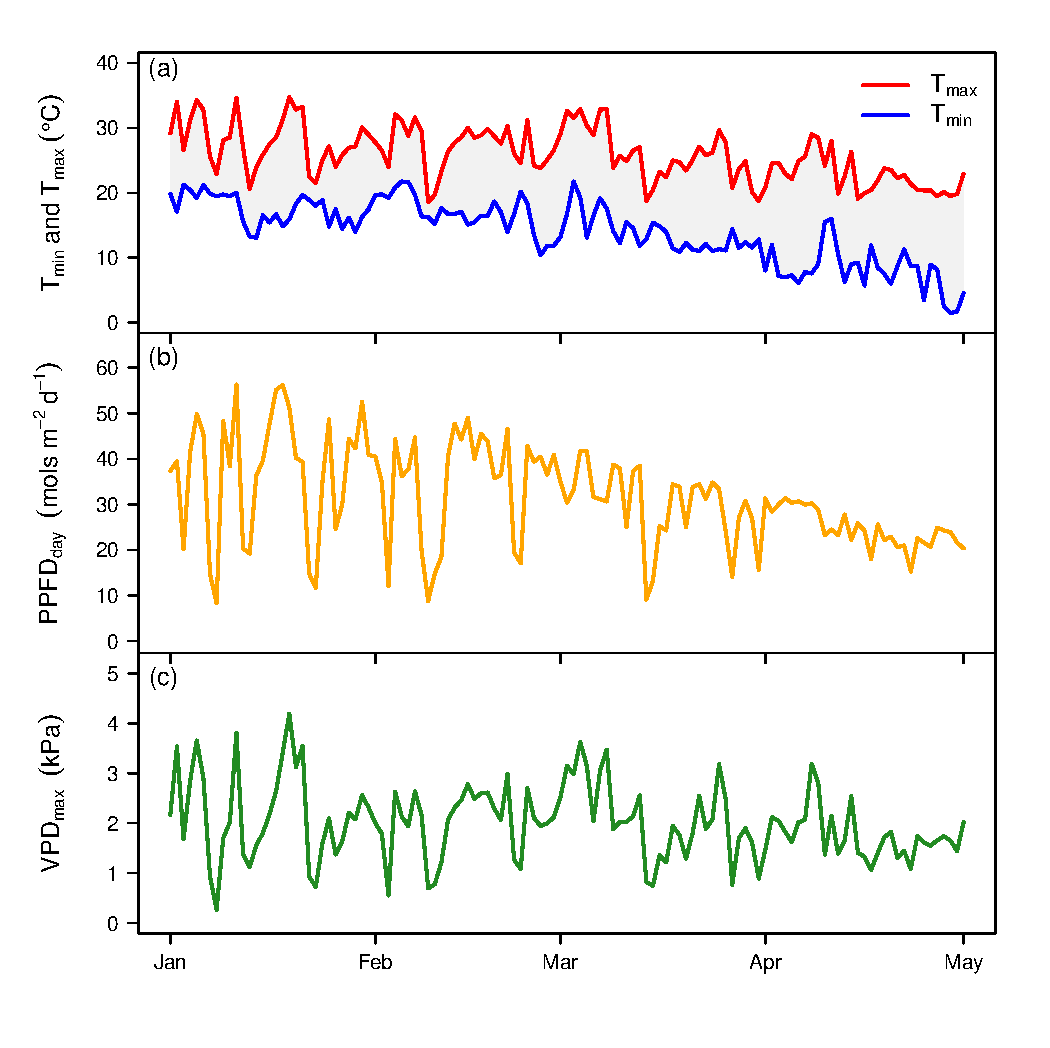
\includegraphics{airvars.pdf}
    \caption{airvariables}
    \label{fig:figure1}
\end{figure}

%allometry figure
\begin{figure}[h!]
    \centering
    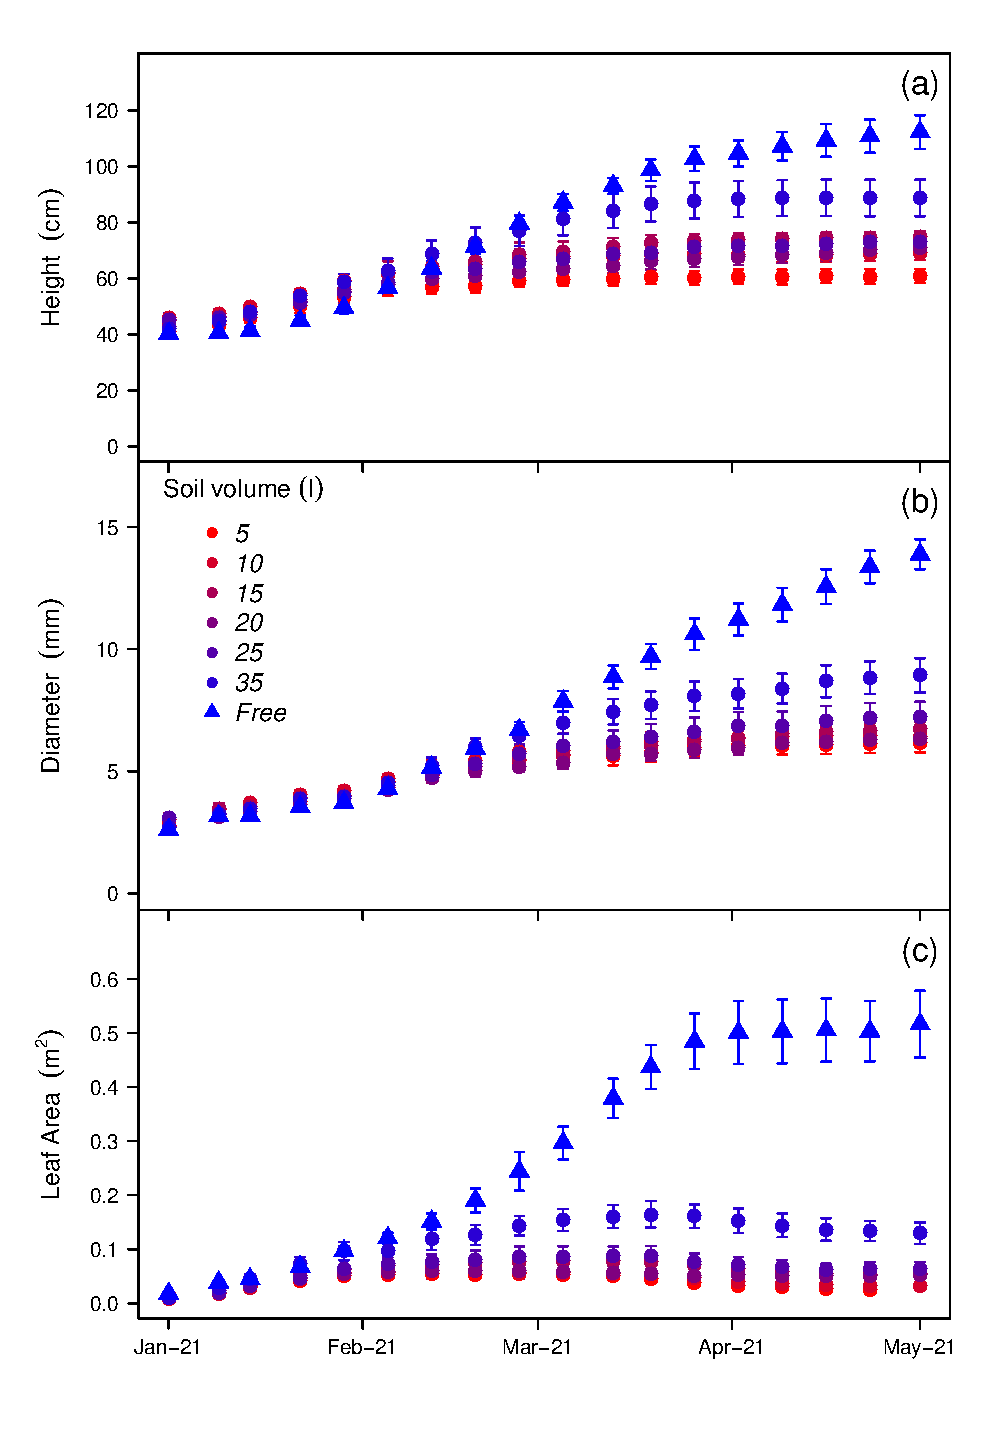
\includegraphics{allometry.pdf}
    \caption{allometry}
    \label{fig:figure2}
\end{figure}

%asat figure
\begin{figure}[h!]
    \centering
    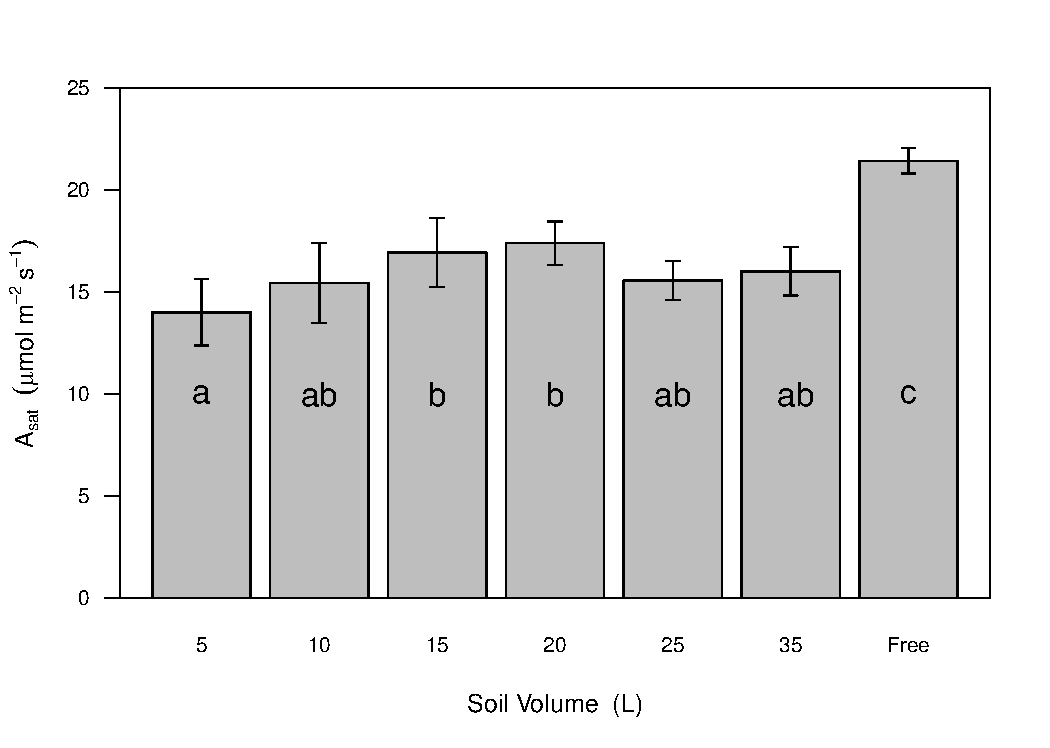
\includegraphics{Asat.pdf}
    \caption{asat}
    \label{fig:figure3}
\end{figure}

%partitioning figure
\begin{figure}[h!]
    \centering
    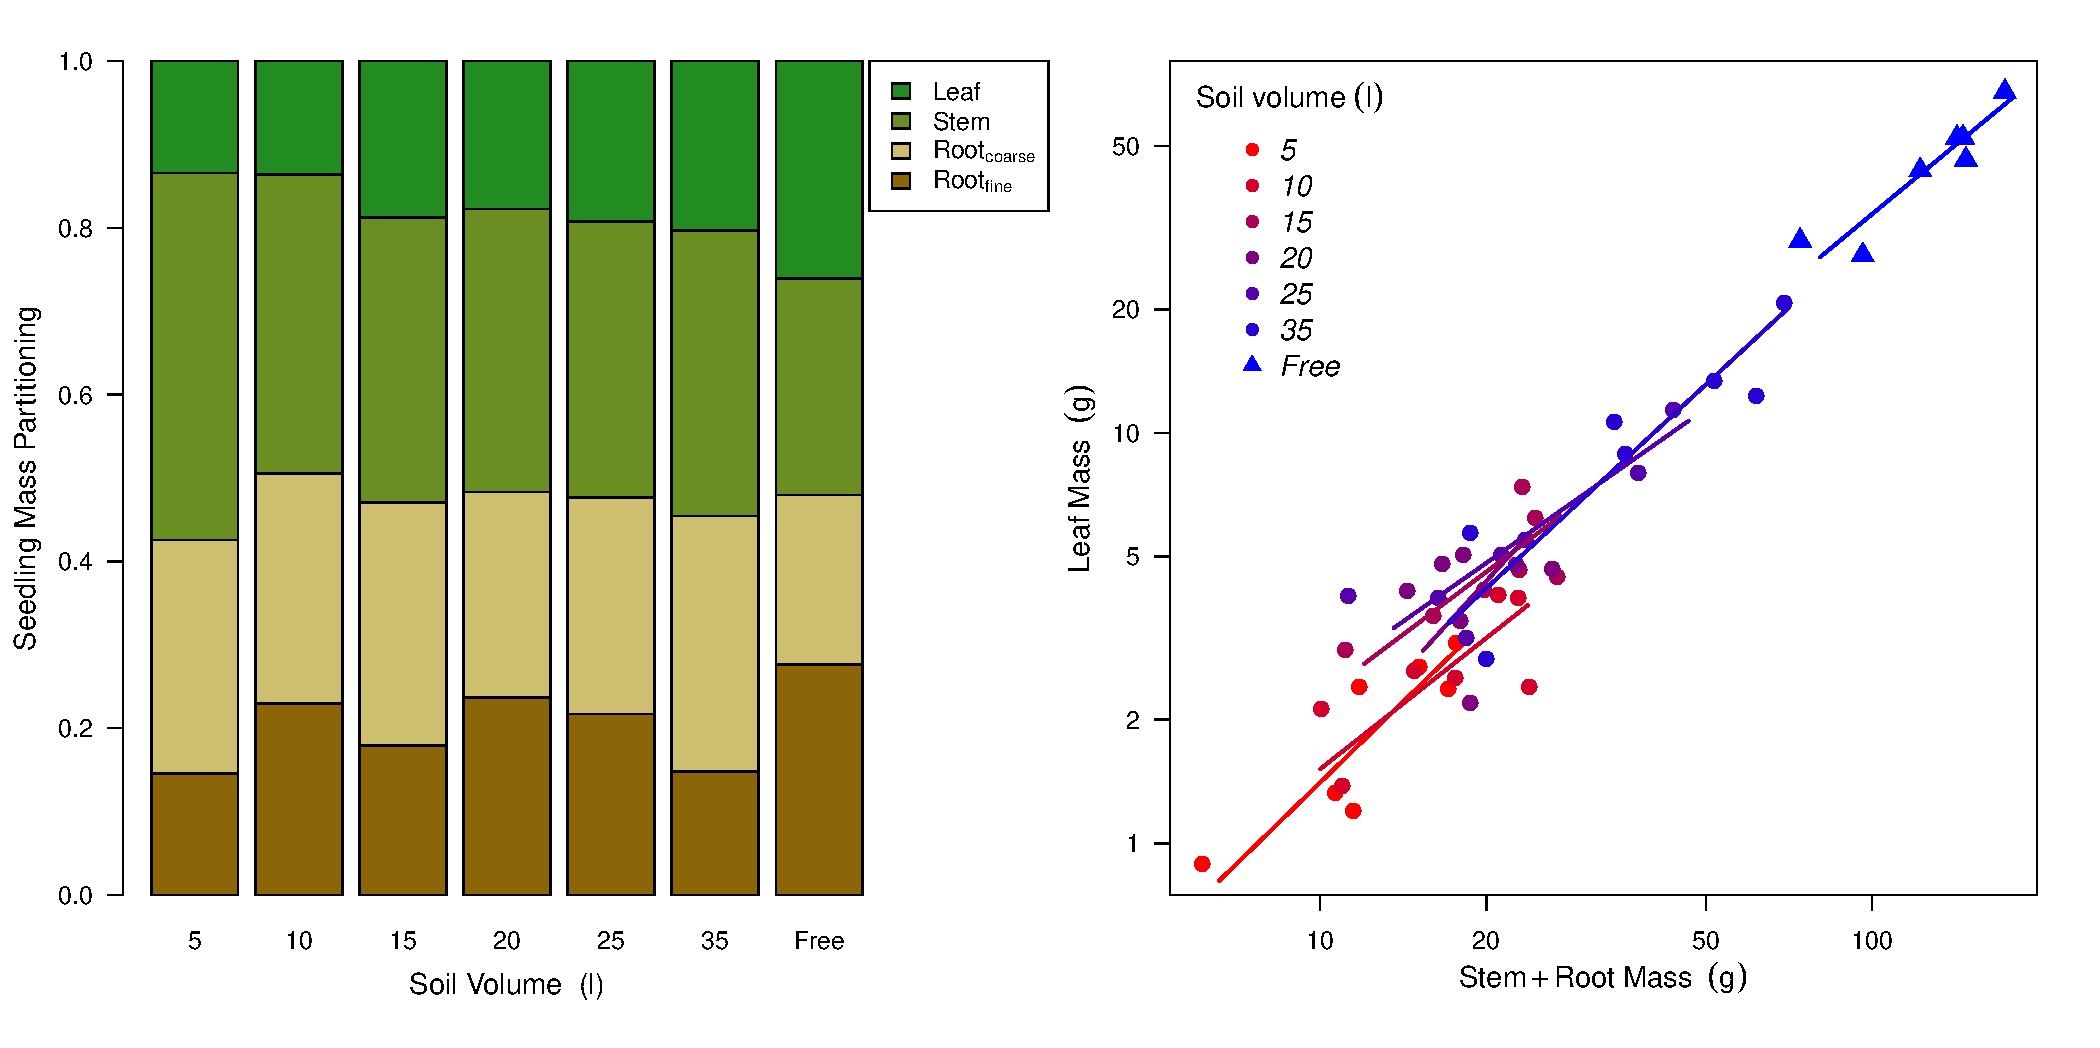
\includegraphics{massfractions.pdf}
    \caption{mass fractions}
    \label{fig:figure4}
\end{figure}

%photochem figure
\begin{figure}[h!]
    \centering
    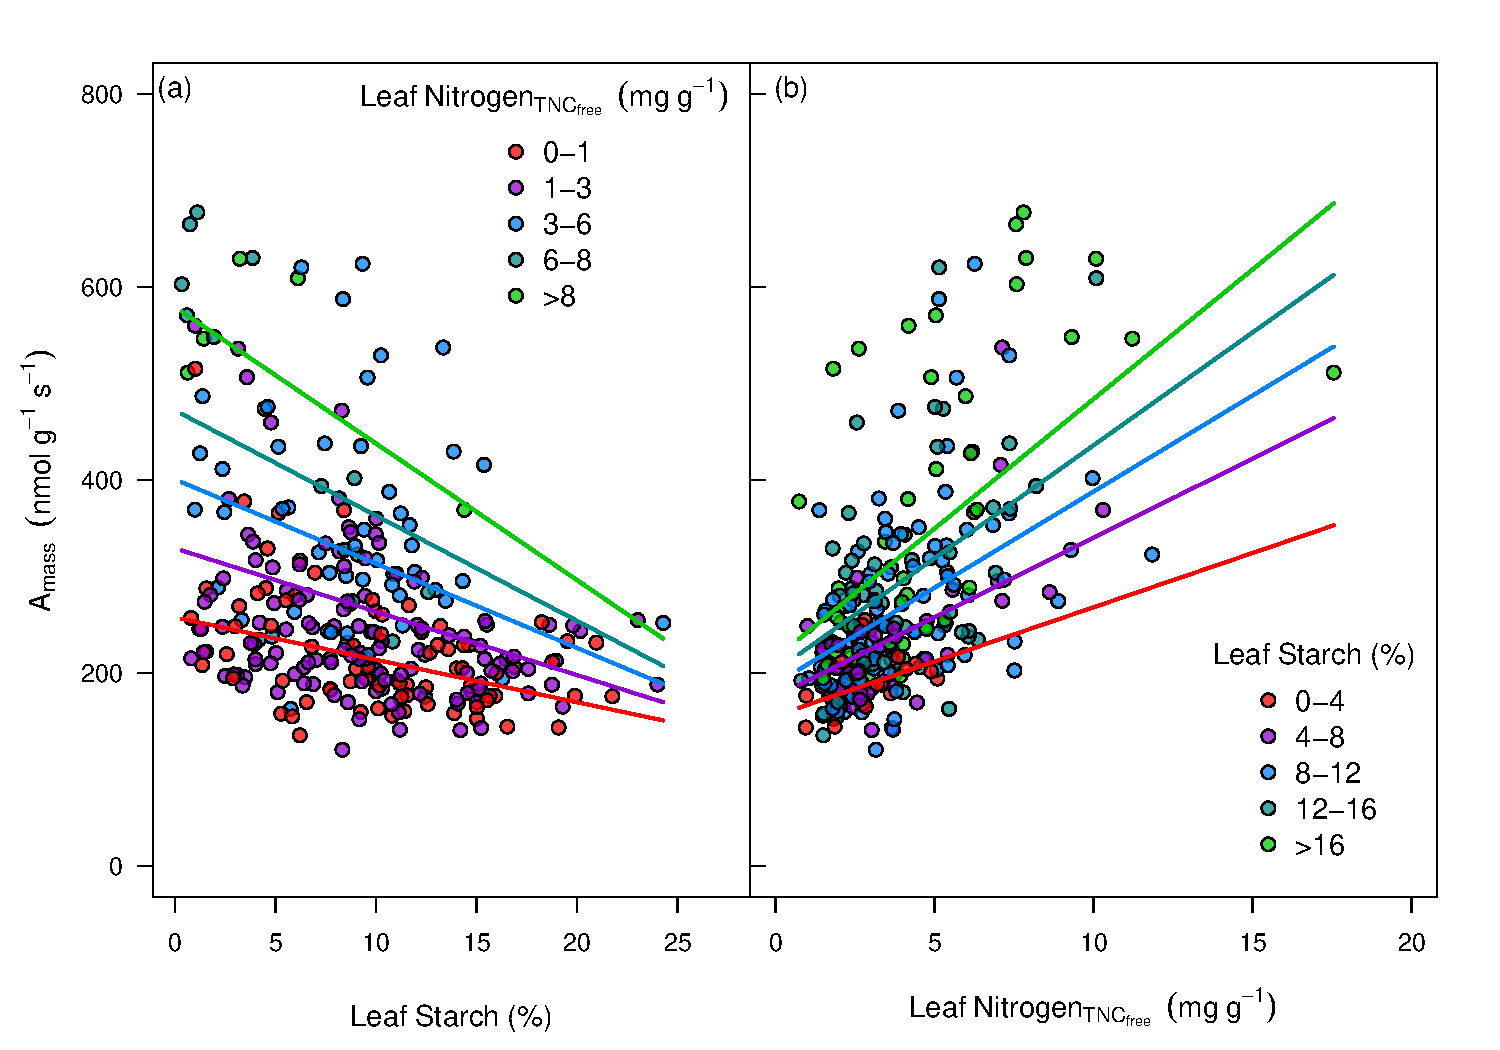
\includegraphics{A_leafchem.pdf}
    \caption{photochem}
    \label{fig:figure5}
\end{figure}

%model base figure
\begin{figure}[h!]
    \centering
    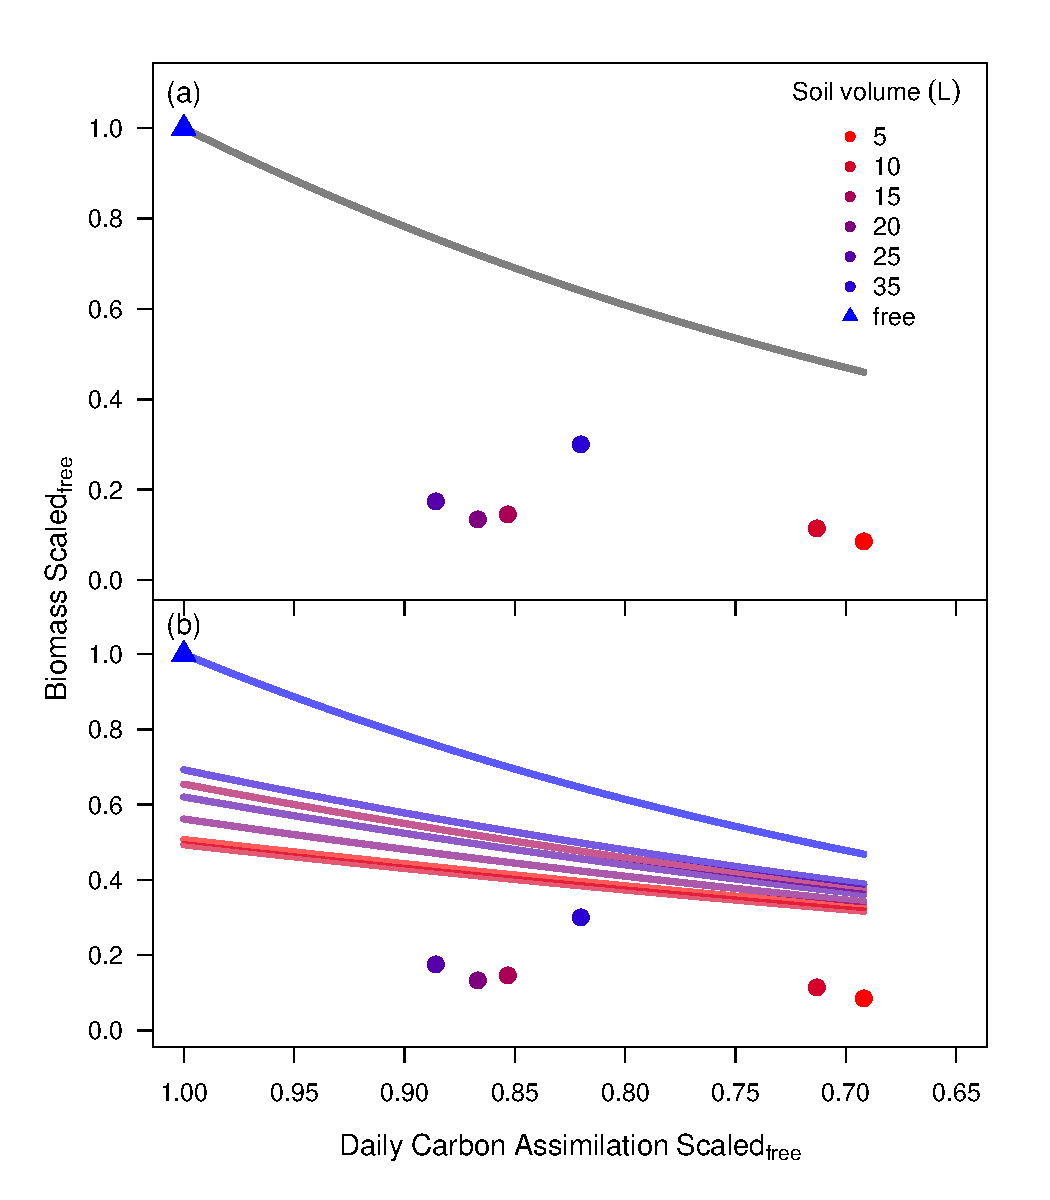
\includegraphics{gC_day.pdf}
    \caption{gcday}
    \label{fig:figure6}
\end{figure}


\clearpage
\section{Supporting Information Figures}
% Supporting information. Make sure Figures continue with Fig S1 etc.

\renewcommand\thefigure{S\arabic{figure}}    
\setcounter{figure}{0}   


\begin{figure}[h!]
    \centering
    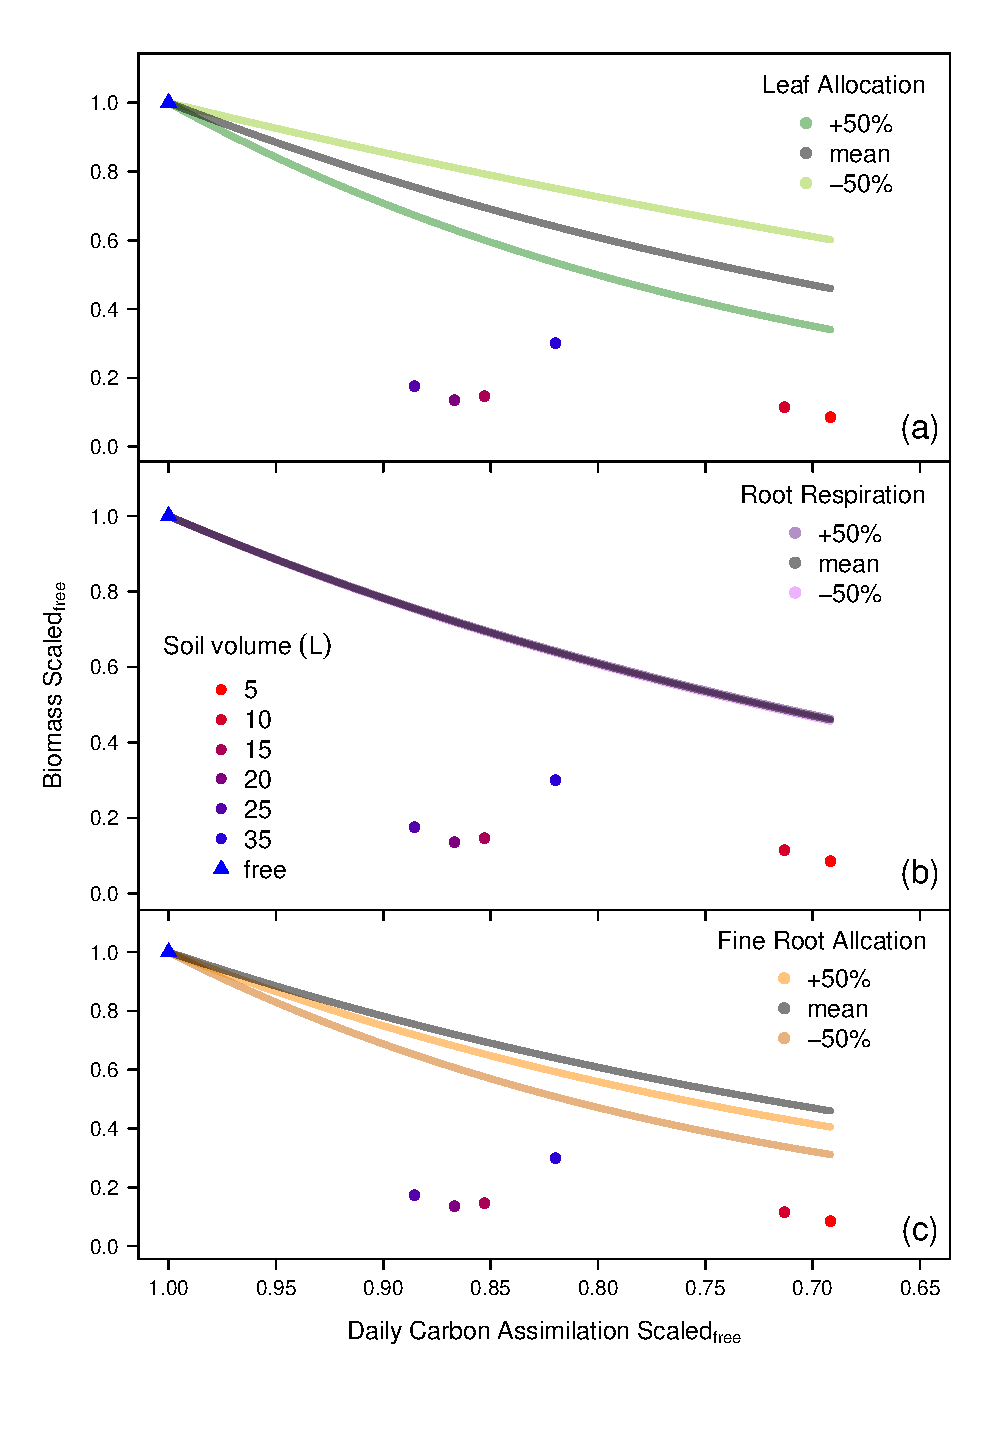
\includegraphics[width=0.99\textwidth]{gc_Day_scenario.pdf}
    \caption{scenarios}
    \label{fig:figureSI1}
\end{figure}

\clearpage
\bibliography{pve_cites}

\end{document}



